\documentclass[a4paper, 12pt]{article}


%%%%%%%%%%%%%%%%%%
%   Liste des packages utilisés  %
%%%%%%%%%%%%%%%%%%

\usepackage{float}
\usepackage{lmodern} %Pack de police
\usepackage{graphicx}
\usepackage[utf8x]{inputenc}
\usepackage[T1]{fontenc}
\usepackage[francais]{babel}
\usepackage{caption}
\usepackage[top=2cm, bottom=2cm,left=2cm, right=2cm]{geometry}
\usepackage{setspace}
\usepackage{fancyhdr}
\usepackage{titlesec, blindtext, color} % titres spéciaux + couleur pour les chapter

% on transforme les chapters en juste le numéro suivi du titre, avec un barre grisse
\definecolor{gray75}{gray}{0.75}
\newcommand{\hsp}{\hspace{20pt}}
\titleformat{\chapter}[hang]{\Huge\bfseries}{\thechapter\hsp\textcolor{gray75}{|}\hsp}{0pt}{\Huge\bfseries}

%Définition du style des bords de page
\pagestyle{fancy}
\lhead{}
\chead{}
\rhead{\rightmark}
\lfoot{Groupe n\up{o}2}
\cfoot{}
\rfoot{Page \thepage}

\begin{document}

%%%%%%%%%%%
%  Page de garde  %
%%%%%%%%%%%
\begin{titlepage}
	\begin{center}
	
		\begin{spacing}{1.5}
			Projet Picross\\
			\vspace*{\fill}
		\end{spacing}
	\end{center}
	\begin{figure}
		
\includegraphics[width=3cm]{logo.png}
	\end{figure}
	\begin{center}
		\begin{spacing}{2}
		    \hrule \vspace{1cm}
			\textbf{\Huge Application de création et d'aide à la résolution de puzzle \textit{picross}}\\[0.5cm]
			\textbf{\huge Cahier des charges} \\
			\vspace*{\fill}
			\hrule \vspace{1cm}
			\textbf{Groupe n\up{o}2}
		\end{spacing}

		\begin{spacing}{1.15}
			\large
			\textsc{Brinon} Baptiste\\
			\textsc{Brocherieux} Thibault\\
			\textsc{Cohen} Mehdi\\
			\textsc{Debonne} Valentin\\
			\textsc{Lardy} Anthony\\
			\textsc{Mottier} Emeric\\
			\textsc{Pastouret} Gilles\\
			\textsc{Pelloin} Valentin\\
			\vspace*{\fill}
			%\textbf{Groupe n\up{o}2} \\
			\textnormal{\large Licence Informatique\\ Le Mans Université\\ \today}
		\end{spacing}
		
	\end{center}
\end{titlepage}

%%%%%%%%%%
%    Sommaire    %
%%%%%%%%%%
\renewcommand{\contentsname}{Sommaire}
\tableofcontents

\newpage
\section{Présentation}
\vspace*{0.5cm}
	\subsection{Introduction}

		Dans le cadre de l'unité d'enseignement « Génie logiciel 2 » de la Licence d'informatique de Le Mans Université, les étudiants de troisième année sont amenés à travailler sur le développement d'une application.
		
		Ce document décrit le contexte, les besoins fonctionnels, les objectifs et les contraintes définis par les clients. Un premier découpage des étapes nécessaires à la réalisation du projet donne lieu, dans le document, à un planning prévisionnel.

	
 	\subsection{Objectifs de l'application}	
 	
		Nous devons réaliser un jeu de type picross, aussi appelé \textit{nonogramme}, \textit{logigramme} ou \textit{hanjie}, qui, au même titre que les mots croisés ou le Sudoku, nécessite une réflexion plus ou moins importante en fonction de la difficulté des grilles.
		
		L'application permet ainsi à un utilisateur de résoudre des grilles, et de l'aider dans leur réalisation.

	\subsection{Règles du \textit{picross}}
	
		Le picross est un jeu de type puzzle. Le jeu consiste à découvrir un dessin sur une grille de taille variable (5x5, 10x10, etc.), en noircissant des cases à l'aide d'indices donnés en marge.
		Les nombres indiqués permettent d'identifier la longueur des blocs de cases à colorier sur la ligne ou colonne. Ces indices se lisent de haut en bas, et de gauche à droite.
		
		Chaque groupe de cases doit être séparé des autres d'au moins une case blanche.
		
		Ci-dessous, un exemple de grille résolue :
		
	\begin{figure}[H]
		\centering
		\caption{Exemple de grille résolue}
		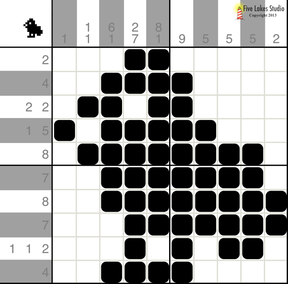
\includegraphics[width=8cm]{picross.png}
	\end{figure}
	
	\newpage	
\section{Spécification des besoins}
\vspace*{0.5cm}

		\subsection{Modes de jeu}
		
			L'application est composée de différents modes de jeu :
			\begin{itemize}
            	\item Le didactitiel : permet la découverte du jeu.
            	\item Le mode classique : divisé en plusieurs chapitres de difficultés variables.
            	\item Le mode évolutif : composé de plusieurs grilles s'élargissant au cours de la partie.
        	\end{itemize}

	    \subsubsection{Didacticiel}
	    
		    Un chapitre de l'application est présent comme didacticiel. Ce chapitre est optionnel et permet aux joueurs   débutants de se familiariser avec les règles du \textit{picross} ainsi qu'à l'utilisation de l'application. Il consiste en plusieurs parties guidées. Les grilles du didacticiel font découvrir les notions du jeu, telles que :
		    \begin{itemize}
            	\item colorier et cocher une case,
            	\item utiliser les aides et les hypothèses,
            	\item acquérir les automatismes de résolution,
        	\end{itemize}
		    en expliquant au joueur les actions à réaliser étape par étape afin de finir la grille. L'application contient également un rappel des règles générales du \textit{picross}.
		    
		\subsubsection{Mode classique}
		
		    Le mode classique est un mode permettant au joueur de compléter des grilles de tailles variées, allant de 5x5 à 20x20, et de difficultés croissantes, plus le joueur progresse dans le jeu.
		    
		    Au commencement, seul le premier chapitre est débloqué. Le joueur peut débloquer les chapitres suivant en collectant suffisamment d'étoiles, qu'il peut gagner à la résolution de chaque grille.
		    
		    La difficulté d'une grille est caractérisée par sa taille ainsi que le nombre de ses indices. Plus une grille est grande, en possédant de nombreux indices faibles, plus elle est difficile à être résolue.
		    
		\subsubsection{Mode évolutif}
		
		    Le mode évolutif est un mode permettant au joueur de compléter des grilles qui croissent au cours de la partie.
		    
		    Ainsi, le joueur commencera sur une grille de taille 5x5. Une fois celle-ci résolue, elle évoluera en grille de taille 10x10, tout en gardant ce que le joueur avait déjà réalisé. 
		    
		    Ce processus se répète jusqu'à la résolution totale de la grille, afin de découvrir une image.
			
\newpage

		\subsection{Aides}
		
			Un système d'aide est intégré au jeu, permettant au joueur d'être assisté lorsque ce dernier est dans l'incapacité de progresser. Il y de ce fait plusieurs types d'aides, dépendant de la difficulté des chapitres.
			\begin{itemize}
			\item Pour un chapitre facile, l'aide permet de colorier une ligne ou une colonne entière. 
			
			\item Pour un chapitre de difficulté moyenne, l'aide permet uniquement de colorier un groupe de bloc d'une ligne ou d'une colonne. 
			
			\item Pour un chapitre difficile, l'aide permet d'indiquer la ligne ou la colonne où se trouve une case correcte non coloriée. 
			\end{itemize}
			
			Plus le joueur avance dans des chapitres difficiles, moins celui-ci est autorisé à utiliser d'aides au cours de sa partie de \textit{picross}. 

		\subsection{Hypothèses}	
		
			À tout moment durant une partie, le joueur peut décider d'utiliser un système d'hypothèses. 
			
			Ceci permet au joueur d'émettre des suppositions quant à la réalisation d'une grille, lorsqu'il n'est pas sûr de lui. Le système actif, permet de colorier les cases d'une autre couleur, représentant un niveau d'hypothèse. Ce système est limité à 5 niveaux, pour un souci de clarté, chacun représentés par une couleur différente.
			
			Si le joueur se rend compte que l'une de ses hypothèses est fausse, il peut l'annuler. Cela a pour effet de supprimer toutes les autres hypothèses posées après celle annulée. Ceci le fait donc revenir à l'état de l'hypothèse précédente.
			
			En revanche, il peut décider qu'une hypothèse est vraie. Dans ce cas, toutes les autres hypothèses qui interviennent avant celle-ci le deviennent aussi. Les cases colorées changent alors de couleur, et deviennent des cases normales.

		\subsection{Score}
		
			On évalue le score d'un joueur sur une grille par le nombre d'étoiles obtenues au total. Un joueur peut gagner quatre étoiles par grille au maximum. Le nombre d'étoiles décernées au joueur, lorsque celui-ci termine le niveau, est calculé en fonction du temps qu'il a mis à résoudre la grille. Le système d'hypothèses n'impacte pas le score obtenu. 
			
			Les chapitres du jeu se débloquent automatiquement, une fois que le nombre total d'étoiles requis est atteint par le joueur pour les déverrouiller.
			
			Plus un chapitre contient de grilles difficiles, plus le nombre d'étoiles requis pour le débloquer est élevé.
			
			Durant une partie, le joueur peut mettre le jeu en pause à n'importe quel moment. Le chronomètre est alors arrêté, et la grille est masquée, rendant impossible toute interaction avec.
\newpage
		\subsection{Statistiques}
		
			En plus du score, l'application garde en mémoire certaines statistiques associées au joueur ainsi qu'aux grilles. 
			
			Les statistiques liées au joueur comportent son score total, le nombre de niveaux et de chapitres accomplis. 
		
			Les statistiques associées à chaque grilles sont le meilleur temps effectué par le joueur, ainsi que le nombre d'aides utilisées.

		\subsection{Interface homme-machine}
		
			L'utilisateur possède le choix de jouer à la souris, au clavier, ou même les deux à la fois.
			
			Il peut également sélectionner un groupe de cases verticale ou horizontale et le colorier d'un seul coup, à la souris comme au clavier. Lors de cette action, le nombre de cases sélectionnées est affiché pour aider le joueur. 
			
			L'application sauvegarde automatiquement la partie après chaque action du joueur afin de pouvoir reprendre n'importe quelle grille à tout moment.
			
			L'application est disponible pour le moment en français et en anglais, avec un système permettant de rajouter des langues supplémentaires ultérieurement.

\newpage
\section{Spécification des contraintes}
\vspace*{0.5cm}
	\subsection{Conception}
	
		Le client demande que le logiciel soit réalisé en Ruby, et que la documentation soit engendrée via \textit{RDoc}. Celle-ci sera remise avec les livrables. L'interface doit être programmée avec \textit{GTK}.
		
	\subsection{Cartes et interface}
	
		Une carte est composée de cases noires, représentant celles validées par le joueur, et blanches, afin de ne pas les confondre avec les cases colorées du système d'hypothèses.
		La joueur à également la possibilité de marquer une case d'une croix, afin d'indiquer qu'elle doit rester vide.
		
		La grille doit prendre suffisamment de place sur la fenêtre de manière à être facilement lisible et jouable malgré l'importante quantité de chiffres. La taille maximale d'une grille est de 25x25.
		
		Lorsqu'une grille est complétée, celle-ci représente une forme évocatrice, telle qu'un objet ou un animal.
	
	\subsection{Limitation de l'aide}
	
		L'utilisation de l'aide n'est pas limité. Cependant, un temps de pénalité est attribué lors de l'utilisation d'une aide. Ceci impacte donc les étoiles remportées à la fin de la partie. 
		
		La pénalité et le temps de jeu sont indiqués séparément. Le total des deux indique le temps final passé sur la grille, servant à calculer le score obtenu. 
		
		Le joueur possède également des aides n'infligeant pas de pénalité. Celles-ci sont obtenues lorsque le joueur complète un niveau ou un chapitre. 
	
	\subsection{Gameplay}
	
		Lors d'une pause, le chronomètre est arrêté. Le joueur aurait la possibilité de résoudre la grille sans que le temps ne défile, brisant ainsi le système de scores. 
		Pour éviter cela, on effectue un masquage de la grille.
		
	\subsection{Didacticiel}
	
		Le didacticiel est un chapitre spécial du jeu accessible à n'importe quel moment. Il se trouve sur le menu principal. 
		Il n'est pas obligatoire, mais recommandé pour un nouveau joueur afin d'apprendre les bases du jeu. Ce chapitre octroie tout de même des étoiles.
		
		Il contient le nécessaire pour expliquer toutes les règles ainsi que le fonctionnement du logiciel (explication de l'interface, système de score).

\newpage
	\subsection{Sauvegardes \& hypothèses}
	
		Les sauvegardes sont réalisées automatiquement. L'utilisateur ne peut donc pas réaliser de sauvegardes manuelles. 
		
		Lors d'une sauvegarde, l'ensemble des hypothèses de la grille en cours est également enregistré. Le nombre d'hypothèses est limité afin de conserver la clarté de la carte. Le maximum est fixé à 5 hypothèses simultanées.
		
		Ainsi, lorsque le joueur souhaite reprendre sa partie, il retrouve son avancée telle qu'il l'a laissée lors de son dernier temps de jeu.
	
	\subsection{Délais}
	
		Le logiciel doit être terminé pour le Jeudi 12 Avril 2018, soit approximativement 3 mois pour la réalisation de ce projet. L'organisation de ce temps est représentée sur le diagramme de \textit{Gantt} suivant :

	\begin{figure}[H]
		\centering
		\caption{Diagramme de \textit{Gantt} général du projet}
		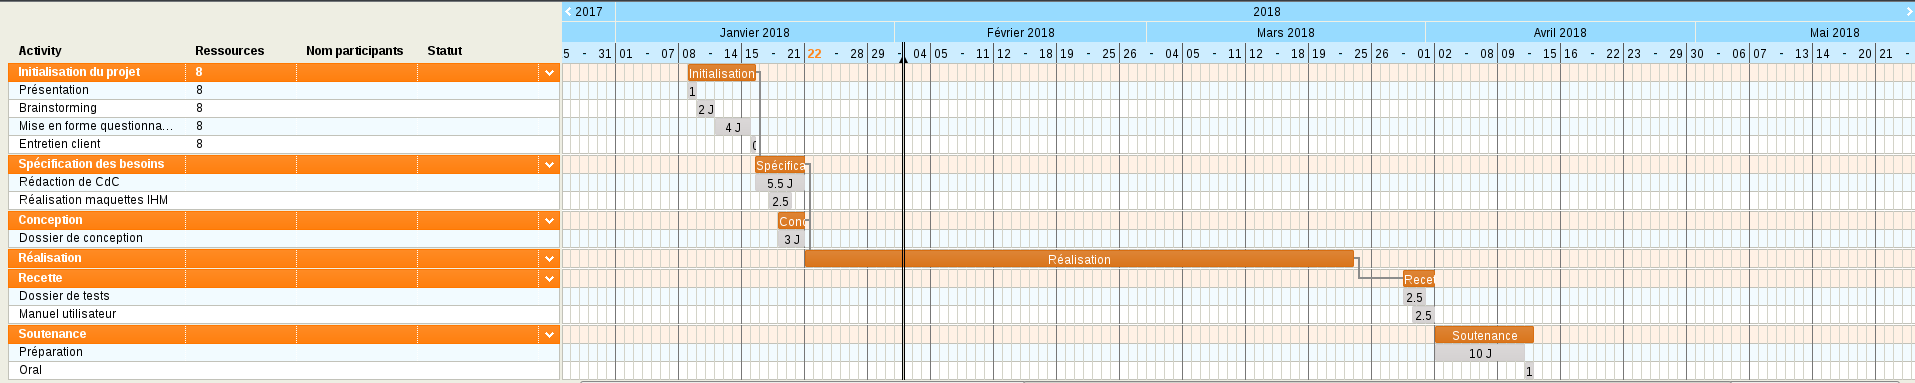
\includegraphics[width=17cm]{ganttGeneral.png}
	\end{figure}	     
		
		Un diagramme de \textit{Gantt} détaillé de la phase de réalisation est donné dans le cahier d'analyse et de conception.

\newpage		
\section{Livrables}
\vspace*{0.5cm}
	Les livrables rendus à l'issue de ce projet sont :
	\begin{itemize}
	\item Le cahier des charges
	\item Le cahier de conception et d'analyse
	\item Le logiciel fonctionnel respectant le cahier des charges
	\item La documentation (\textit{RDoc})
	\item Le manuel utilisateur
	\end{itemize}
		
%	``I always thought something was fundamentally wrong with the universe'' \citep{adams1995hitchhiker}	
		\bibliographystyle{plain}
		\bibliography{references}

\end{document}
